\vspace*{\fill}
\begin{center}
  {\huge\textbf{Обжора}}

  \vspace{1.5em}  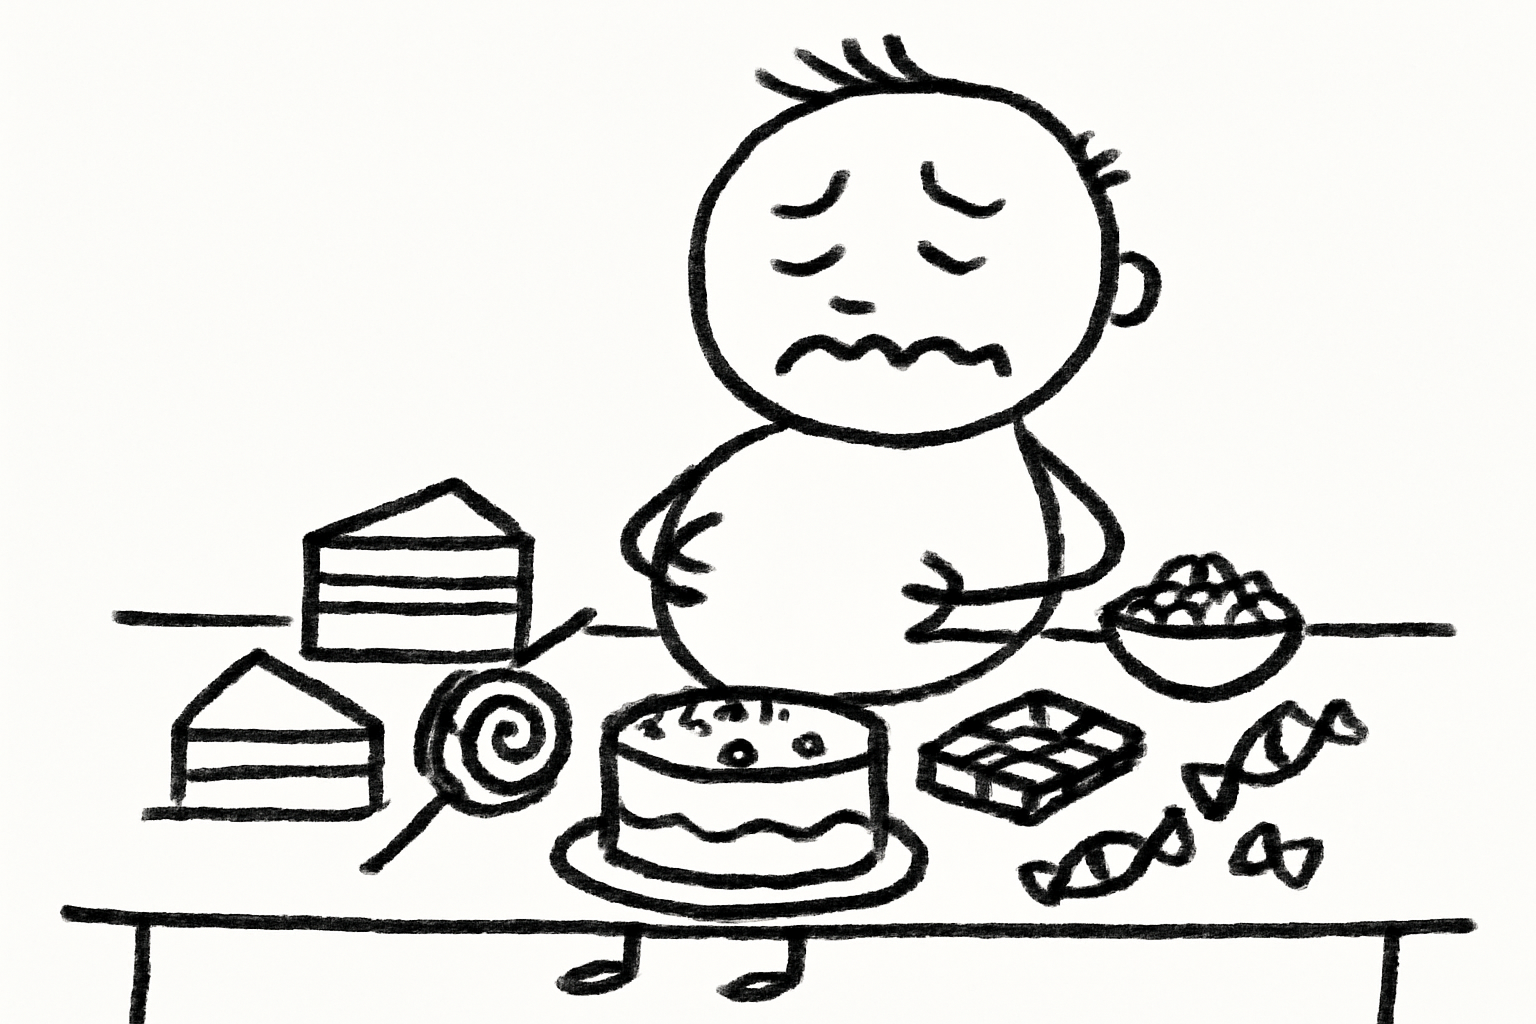
\includegraphics[width=0.7\textwidth]{pictures/obzhora.png}
  \vspace{4em}
  \parbox{0.6\textwidth}{
    \LARGE
    \begin{spacing}{1.2}
      Жил-был мальчик-обжора Петя,\\
      Ел он все на белом свете.\\
      Торт, конфеты, шоколад -\\
      Съесть все это был он рад!\\
      \\
      Но однажды заболел,\\
      Слишком много он поел.\\
      Теперь кушает немножко,\\
      Бережет свой животик, крошка! %
    \end{spacing}
      
  }
\end{center}
\vspace*{\fill}